%!TEX encoding = UTF-8 Unicode
%!TEX root = ../compendium2.tex

\Lab{\LabWeekEIGHT}

\begin{Goals}
\item Kunna skapa och använda matriser.
\item Kunna iterera över matriser med nästlade for-loopar.
\item Träna på algoritmkonstruktion.
\item Använda en integrerad utvecklingsmiljö (IDE).
\end{Goals}

\begin{Preparations}
\item Gör övning {\tt \ExeWeekEIGHT} i kapitel \ref{chapter:W08}.

\item Läs igenom hela laborationen och studera den befintliga koden i \code{workspace}.

\item Skriv pseudokod för metoderna \code{draw} och {walk}, som beskrivs nedan.

\item Läs appendix \ref{appendix:ide} och välj vilken IDE du ska använda (ScalaIDE/Eclipse eller IntelliJ IDEA). Säkerställ att du får igång en av dessa utvecklingsmijöer genom att köra hello-world-exemplet och sedan ladda ner och importera kursens workspace enligt instruktionerna i appendix \ref{appendix:ide}.
\end{Preparations}

\subsection{Bakgrund}

En labyrint är ett rum som har en ingång och en utgång.  I denna laboration ska du rita labyrinter och sedan implementera en algoritm för att hitta ut ur labyrinter.

För våra labyrinter gäller följande begränsningar: Ingången är alltid längst ner i labyrinten, och utgången alltid högst upp. Dessutom är alla väggar parallella med antingen x-axeln eller y-axeln.

Man kan representera en sådan labyrint med hjälp av en boolesk matris, så som visas i figur \ref{maze:figboolmatrix}. Varje element i matrisen motsvarar en ruta i labyrinten. Värdet \code{true} i matrisen representerar att det finns en vägg på motsvarande ruta i labyrinten och \code{false} representerar en öppen ruta där man kan gå.

\begin{figure}[h]
	\begin{center}
		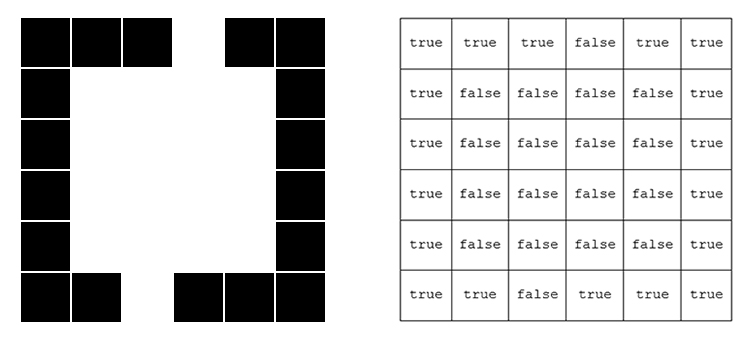
\includegraphics[width=0.7\textwidth]{../img/w09-lab/MazeAndMatrix.jpg}
	\end{center}
	\caption{Exempel på en matrisrepresentation av en enkel labyrint.}
	\label{maze:figboolmatrix}
\end{figure}

Det finns många olika sätt att ta sig igenom en labyrint.\footnote{Om du är intresserad, läs om olika algoritmer för att ta sig igenom en labyrint här: \url{https://en.wikipedia.org/wiki/Maze\_solving\_algorithm}} Ett enkelt sätt att hitta utgången, som kanske inte följer närmsta vägen, är att hålla vänster hand i vänster vägg och följa väggen med handen tills man når öppningen. Detta fungerar för alla labyrinter där väggarna från ingången till utgången är sammankopplade.

När man går igenom labyrinten finns det fyra olika riktningar att välja mellan som alla kan beskrivas i antal grader räknat från x-axeln, där höger motsvaras av 0 grader, uppåt motsvaras av 90 grader, vänster av 180 grader och nedåt av 270 grader.

\subsection{Lösningens struktur}

I denna laboration ska du använda den nästan färdiga case-klassen \code{Maze} som representerar en labyrint med hjälp av en boolesk matris implementerad som en \code{Vector[Vector[Boolean]]}.
Du ska implementera klart den påbörjade metoden \code{draw} som ska rita ut matrisen i ett fönster. Till din hjälp har du en lokal metod som ritar ett väggelement i labyrinten.

Du ska även implementera klassen \code{MazeWalker} med metoden \code{walk} som ritar vägen mellan ingången och utgången i en labyrint.

Studera koden för klassen \code{Maze} nedan, speciellt metoden \code{draw}:

\scalainputlisting[basicstyle=\ttfamily\fontsize{9.5}{12}\selectfont,numbers=left]{../workspace/w08_maze/src/main/scala/maze/Maze.scala}

Du har nytta av dessa metoder när du implementerar \code{walk} i \code{MazeWalker}:
\begin{itemize}[noitemsep]
  \item \code{entryPos} ger startpositionen för labyrinten i fönsterkoordinater.
  \item \code{isAtExit} avgör om en position i fönstret är ovanför utgången.
  \item \code{isWallAtLeft} avgör om en position i fönstret har en vägg till vänster givet att man tittar i en viss rikting \code{dir}.
  \item \code{isWallInFront} avgör om en position i fönstret har en vägg rakt fram i den riktning man tittar.
\end{itemize}

När du implmenterar \code{walk} i \code{MazeWalker} ska du använda den färdiga klassen \code{SimpleTurtle} nedan för att rita ut vägen genom labyriten.

\scalainputlisting[basicstyle=\ttfamily\fontsize{10}{12.5}\selectfont,numbers=left]{../workspace/w08_maze/src/main/scala/graphics/SimpleTurtle.scala}

Klassen \code{MazeWalker} nedan har en klassparameter \code{turtle} som är en \code{SimpleTurtle}. Du ska implementera metoden \code{walk} som ritar vägen med hjälp av \code{turtle}. För att man ska hinna se hur sköldpaddan går genom labyrinten \code{maze} ska du skapa en fördröjning med hjälp av ett anrop \code{delay(animationDelay)} vid varje steg som sköldpaddan tar.

\scalainputlisting[basicstyle=\ttfamily\fontsize{10}{12.5}\selectfont,numbers=left]{../workspace/w08_maze/src/main/scala/maze/MazeWalker.scala}

Till din hjälp har du även följande huvudprogram:

\scalainputlisting[basicstyle=\ttfamily\fontsize{9.5}{12.5}\selectfont,numbers=left]{../workspace/w08_maze/src/main/scala/maze/Main.scala}

Det går att köra huvudprogrammet även om du inte gjort klart \code{Maze.draw} och \code{MazeWalker.walk}. Labyrinterna som ligger i \code{resource}-katalogen skrivs ut i terminalen, men ingen labyrint ritas i fönstret och inget rött streck med lösningen visas förrän du gjort klart de saknade delarna.


\subsection{Obligatoriska uppgifter}


\Task Kör igång huvudprogrammet i filen \code{Main.scala} och säkerställ att ditt projekt hittar \code{SimpleWindow} i \code{cslib}, samt att labyrintfilerna i mappen \code{src/resources} hittas av huvudprogrammet och skrivs ut.

\Task Implementera metoden \code{draw} i klassen \code{Maze} så att den ritar upp en labyrint i \texttt{SimpleWindow}, enligt nedan tips:

\begin{itemize}
\item Du behöver skapa en nästlad iteration som går igenom matrisen \texttt{matrix} och undersöker varje element. Om ett element är \texttt{true} ska det ritas upp en bit av en vägg på sin motsvarande plats i \texttt{SimpleWindow} medan om ett element är \texttt{false} ska ingenting ritas upp.
Till din hjälp har du den färdigskrivna metoden \texttt{drawAnotherBrickInTheWall}, som sköter omvandlingen från rader och kolumner i \code{matrix} till fönsterkoordinater i \code{w}.

\item En speciell utmaning är att förstå skillnaden mellan fönstrets koordinater och positionen i den booleska labyrintmatrisen, samt hur översättningen mellan dessa går till. Rita gärna en skiss med exempel på papper för att reda ut detta.
\end{itemize}



\Task Implementera i \code{MazeWalker.walk} en algoritm som får en sköldpadda att ta sig genom en labyrint. Algoritmen ska baseras på idén att alltid hålla vänster hand i väggen (eller sköldpaddsfot i det här fallet). Börja, som förberedelse, att skriva pseudokod för algoritmen, enligt tipsen i följande punkter.


\begin{itemize}

\item För att avgöra om sköldpaddan var en vägg till vänster eller framför sig enligt sin riktning, ska du använda dig av de publika metoder som finns färdiga i \texttt{Maze}.

\item Använd en \code{while}-loop som pågår tills målet är nått. Låt sköldpaddan gå en fönsterpixel i taget med \code{turtle.move(1)} efter eventuell riktningsförändring beroende på väggarnas placering.

\item Gör en fördröjning sist i din loop med hjälp av metoden \code{MazeWalker.delay}, så att du hinner begrunda hur sköldpaddan går i labyrinten. Vid upprepad testning av stora labyrinter är det lämpligt med fördröjningsargumentet 1.

\item Om din algoritm visar sig ha buggar, använd \code{println} för att instrumentera din kod, enligt tipsen som ges i appendix \ref{appendix:debug}. Du kan också använda dig av debuggern i den IDE du valt att använda.

\end{itemize}

\subsection{Frivilliga extrauppgifter}

\Task Skapa din egen labyrint i en textfil kallad \texttt{maze5.txt} i mappen \code{resources}. Kontrollera så att även denna labyrint ritas upp som den ska. Gör gärna en labyrint som du tycker verkar lämplig för människor att lösa, med nästa uppgift i åtanke.


\Task Implementera en metod \code{def humanWalk(maze: Maze): Unit} i klassen \code{MazeWalker} som låter en människa gå i en labyrint genom att styra \code{SimpleTurtle} med tangenterna WASD för upp, vänster, ner, höger. Ge mer poäng desto kortare tid människan använder för att klara labyrinten.

%
% I denna frivilliga extrauppgift ska du generera en slumpmässig labyrint. Du ska använda en förenklad variant av Prims algoritm.\footnote{Om du vill, läs mer om Prims algoritm här: \href{https://en.wikipedia.org/wiki/Prim\%27s_algorithm}{en.wikipedia.org/wiki/Prim\%27s\_algorithm}}
%
% I pseudokoden för vår algoritm, som återfinns nedan, kallas en ruta som inte är en vägg för en \emph{öppen ruta}. Att \emph{öppna en ruta} innebär att en ruta görs om från en vägg till en öppen ruta (om den inte redan är öppen).
%
% Eftersom det i vårt fall endast ska finnas en enda ingång och en enda utgång i labyrinten, måste detta hanteras speciellt.
%
% Först följer en översiktlig beskrivning av algoritmen, sedan pseudokod med mer detaljer.
%
% \begin{enumerate}[noitemsep]
%     \item Skapa en matris helt fylld med väggar.
% 	\item Börja med att slumpmässigt välja en av rutorna i nedersta raden och öppna den rutan, samt rutan ovanför. Detta blir ingången till labyrinten.
% 	\item Applicera väggöppningsalgoritmen som visualiseras i figur \ref{lab:maze:prims-algo-viz} på sida \pageref{lab:maze:prims-algo-viz}. Observera att matrisens ytterkantsväggar inte ska öppnas (förutom ingången och utgången).
% 	\item Slutligen letar vi efter en slumpmässig ruta på näst översta raden som är öppen och öppnar rutan ovanför denna, vilket blir utgången.
% \end{enumerate}
%
% \begin{CodeSmall}
%   def random(rows: Int, cols: Int): Maze = {
%     val maze: Array[Array[Boolean]] = /*initialt en matris med bara väggar*/
%     val wallCandidates: ArrayBuffer[(Int, Int)] = /*initialt inga positioner*/
%
%     // Lägger till omkringliggande vägar runt (row, col) i wallCandidates
%     def addSurroundingWalls(row: Int, col: Int): Unit = /* finns färdig */
%
%     // Ger true om det finns exakt tre väggar runt (row, col)
%     def isThreeWallsAround(row: Int, col: Int): Boolean = /* finns färdig */
%
%     val (startCol, startRow) = (/* slumpmässigt kolumn */, /* sista raden */)
%
%     /* Skapa öppningen */
%     /* Skapa första öppna rutan ovanför öppningen */
%     /* Lägg de väggar som omgärdar första öppna rutan i wallCandidates */
%
%     while (/* finns fler kandidater */) {
%       val rndIndex = /* slumpmässigt index för ngn väggkandidat */
%       val (row, col) = /* position för väggkandidat på plats rndIndex */
%       if (/* exakt tre väggar runt (row,col)*/) {
%         /* öppna denna position */
%         /* lägg till omgärdande väggar i wallCandidates */
%       }
%       /* ta bort väggkandidaten på plats rndIndex ur wallCandidate */
%     }
%
%     /* hitta utgång och öppna den */
%     /* skapa Maze och returnera */
%   }
% \end{CodeSmall}
%
%
% \begin{figure}[H]
% 	\begin{center}
% 		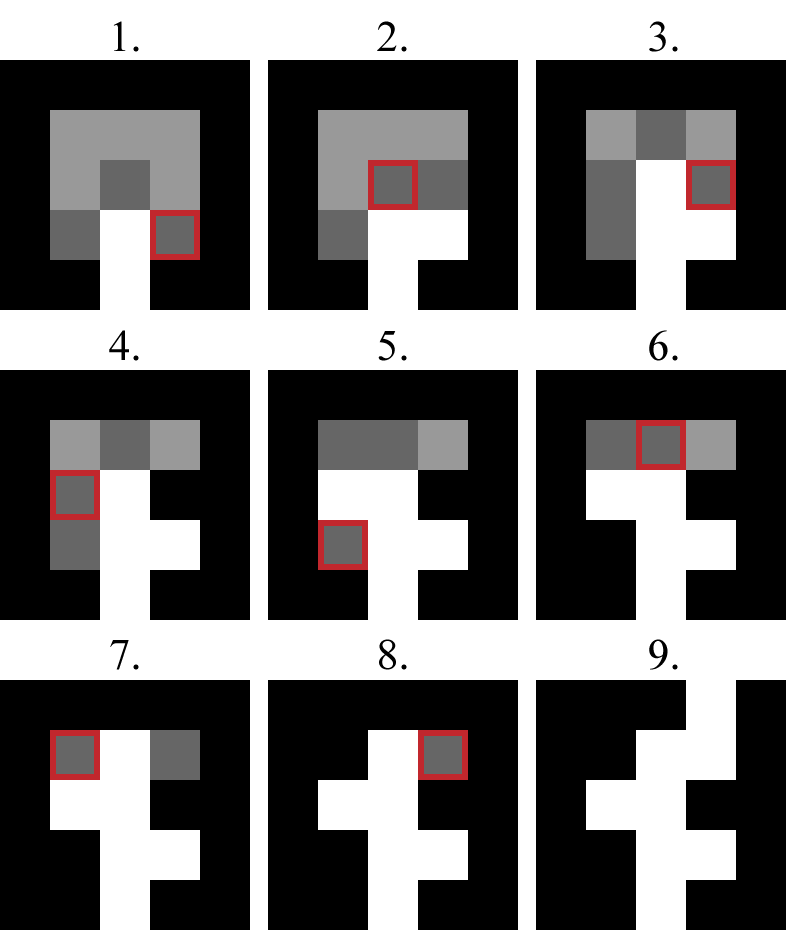
\includegraphics[width=0.45\textwidth]{../img/w09-lab/AlgorithmVisualized.png}
% 	\end{center}
% 	\caption{Visualisering av algoritmen när den genererar en labyrint av storleken 5x5.}
% 	\label{lab:maze:prims-algo-viz}
% \end{figure}
%
%
% \Task Gör färdigt den påbörjade algoritmen som skapar en slumpmässig labyrint enligt nedan.
%
% \Subtask Inspektera ovanstående pseudokod och försök förstå den. Läs igenom uppgifterna nedan. Fråga om något är oklart.
%
% \Subtask Studera de färdiga implementationerna av metoderna \texttt{addSurroundingWalls} och \texttt{isThreeWallsAround} och även den halvfärdiga metoden \texttt{random} i \texttt{Maze} i ditt workspace och se om du kan förstå vad de gör. Det underlättar stort om du kan skapa din egen mentala bild av hur algoritmen fungerar innan du börjar koda, t.ex. genom att rita exempel med papper och penna.
%
% \Subtask Implementera metoden \texttt{random} i \texttt{Maze} som skapar och returnerar en slumpmässigt utformad labyrint med hjälp av pseudokoden ovan. Ta hjälp av metoderna \texttt{addSurroundingWalls} och \texttt{isThreeWallsAround}.
%
% \Subtask Skapa en slumpmässig labyrint i ditt huvudprogram genom att anropa metoden \texttt{random}. Ett bra värde att använda när du anropar metoden är något tal mellan 20 och 100. Det vill säga anropa metoden genom att exempelvis skriva \texttt{random(50, 50)}. När du har slumpat fram en labyrint, testa att låta din sköldpadda gå igenom labyrinten och se om den lyckas!
%
% \Subtask Om din algoritm har buggar, använd \code{println} för att instrumentera din kod, enligt tipsen som ges i appendix \ref{appendix:debug}, i arbetet med att åtgärda buggarna.
%
% \begin{figure}[h]
% 	\begin{center}
% 		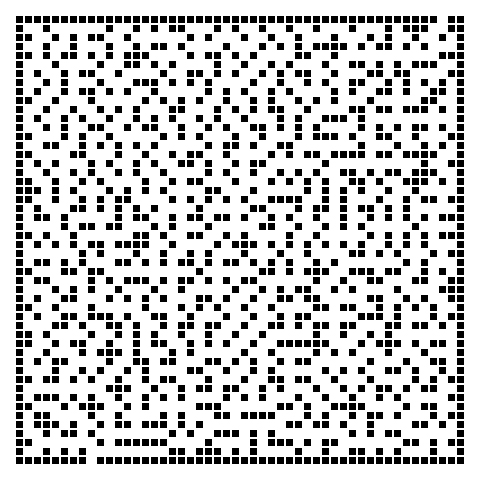
\includegraphics[width=1.0\textwidth]{../img/w09-lab/RandomMaze.jpg}
% 	\end{center}
% 	\caption{Ett exempel på hur en slumpmässigt utformad labyrint kan se ut.}
% \end{figure}
